% ============================================================================
%  Problems: มุมและเส้นขนาน (Angles & Parallel Lines)
%  Ordered from easy (basic) → intermediate.
%  Shared by exercise.tex and answer-key.tex
% ============================================================================

% --- Part 1: พื้นฐาน (Basic) ---
\examsection{ตอนที่ 1: พื้นฐาน — ชนิดของมุมและมุมประกอบ}

\problem{
  มุมหนึ่งมีขนาด $35^\circ$ จงหาขนาดของมุมประกอบฉาก (complement) ของมุมนี้
}{
  มุมประกอบฉาก $= 90^\circ - 35^\circ = 55^\circ$
}

\problem{
  มุมหนึ่งมีขนาด $72^\circ$ จงหาขนาดของมุมประกอบสองฉาก (supplement) ของมุมนี้
}{
  มุมประกอบสองฉาก $= 180^\circ - 72^\circ = 108^\circ$
}

\problem{
  มุมสองมุมเป็นมุมประกอบฉากซึ่งกันและกัน ถ้ามุมหนึ่งใหญ่กว่าอีกมุมหนึ่งอยู่ $20^\circ$
  จงหาขนาดของมุมทั้งสอง
}{
  ให้มุมเล็ก $= x$, มุมใหญ่ $= x + 20^\circ$

  $x + (x + 20^\circ) = 90^\circ$

  $2x = 70^\circ$, $x = 35^\circ$

  มุมทั้งสองคือ $35^\circ$ และ $55^\circ$
}

\problem{
  เส้นตรงสองเส้นตัดกันเกิดมุมมุมหนึ่งมีขนาด $65^\circ$
  จงหาขนาดของมุมตรงข้ามและมุมประชิดของมุมนี้
}{
  มุมตรงข้าม $= 65^\circ$ เท่ากัน

  มุมประชิด $= 180^\circ - 65^\circ = 115^\circ$
}

% --- Part 2: การประยุกต์ (Intermediate) ---
\examsection{ตอนที่ 2: การประยุกต์ — เส้นขนานและสามเหลี่ยม}

\problem{
  เส้นตรง $L_1 \parallel L_2$ และมีเส้นตัดขวางเส้นหนึ่งตัดผ่าน
  ถ้ามุมแย้งมุมหนึ่งมีขนาด $47^\circ$ จงหาขนาดของมุมแย้งอีกมุมหนึ่ง
  และมุมสมนัยกับมุมนั้น
}{
  มุมแย้งอีกมุม $= 47^\circ$ (มุมแย้งเท่ากัน)

  มุมสมนัย $= 47^\circ$ (มุมสมนัยเท่ากัน)
}

\problem{
  เส้นตรง $L_1 \parallel L_2$ และมีเส้นตัดขวางตัดผ่าน
  ถ้ามุมภายในบนด้านเดียวกันของเส้นตัดมุมหนึ่งมีขนาด $112^\circ$
  จงหาขนาดของมุมภายในอีกมุมหนึ่งบนด้านเดียวกัน
}{
  มุมภายในบนด้านเดียวกันรวมกัน $= 180^\circ$

  มุมที่เหลือ $= 180^\circ - 112^\circ = 68^\circ$
}

\problem{
  รูปสามเหลี่ยม $ABC$ มี $\angle A = 38^\circ$ และ $\angle B = 74^\circ$
  จงหาขนาดของ $\angle C$
}{
  $\angle C = 180^\circ - 38^\circ - 74^\circ = 68^\circ$
}

\problem{
  รูปสามเหลี่ยม $ABC$ มี $\angle A = 45^\circ$ และ $\angle B = 55^\circ$
  จงหาขนาดของมุมภายนอกที่เกิดจากการต่อด้าน $AB$ ออกไปที่จุด $B$
}{
  มุมภายนอกที่ $B = \angle A + \angle C$

  $\angle C = 180^\circ - 45^\circ - 55^\circ = 80^\circ$

  มุมภายนอก $= 45^\circ + 80^\circ = 125^\circ$

  [หรือ $180^\circ - 55^\circ = 125^\circ$ ก็ได้]
}

% --- Part 3: ระดับ สอวน. (POSN Level) ---
\examsection{ตอนที่ 3: ระดับข้อสอบ สอวน.}

\problem{
  (ข้อสอบจริงปี 68 ข้อ 25) กำหนด รูปสามเหลี่ยม ABC ให้ D, E, F เป็น จุดบนด้าน AB, BC, AC ตามลำดับ โดยที่ BD=BE และ CE=CF ถ้ามุม $\hat{DEF}=32^\circ$ แล้วมุม $\hat{BAC}$ มีค่าเท่าไร
  \begin{center}
    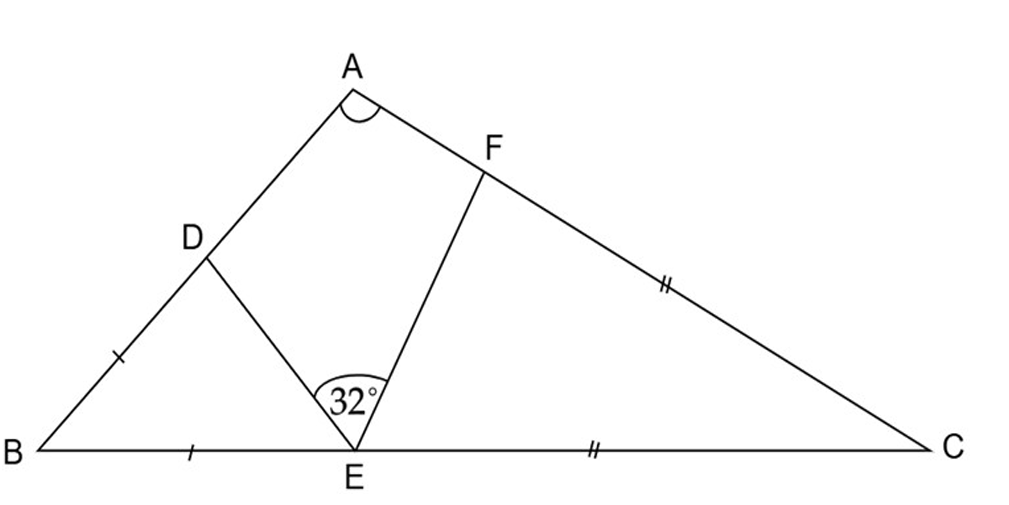
\includegraphics[width=0.5\textwidth]{images/geometry-angles-01.png}
  \end{center}
}{
  $116^\circ$
}